\section{FEATURE IMPORTANCE}
\label{sec:feature_importance}

In predictive modeling for air traffic management, understanding the drivers behind a model's decisions is as critical as its overall accuracy. Figure \ref{fig:feature_importance} presents the aggregated feature importance extracted from the best-performing model, the tuned CatBoost regressor. Because the dataset was one-hot encoded, the importances of the dummy variables were aggregated by their base feature name to reflect the true weight of each categorical variable.

\begin{figure}[htbp]
    \centering
    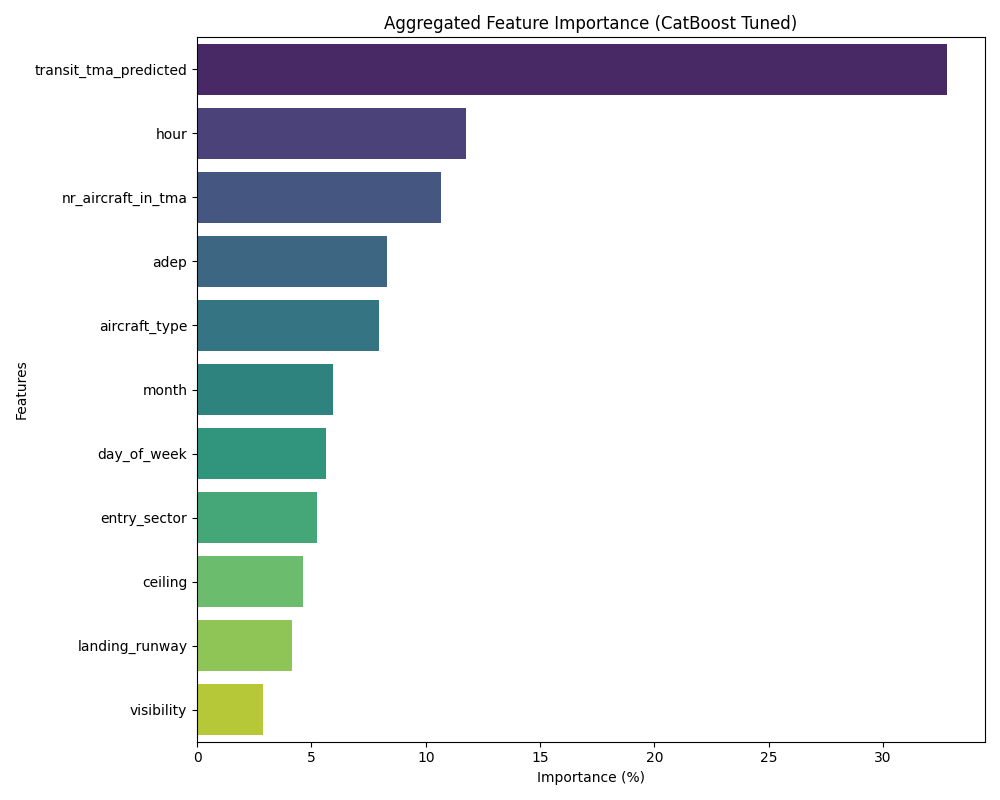
\includegraphics[width=1\linewidth]{images/feature_importance.png}
    \caption{Aggregated feature importance ranking from the tuned CatBoost model.}
    \label{fig:feature_importance}
\end{figure}

The analysis reveals that the moving average of predicted transit time in the TMA (\texttt{transit\_tma\_predicted}) is the most critical explanatory variable, accounting for nearly a third of the model's total predictive power. This outcome underscores the profound impact of airspace congestion on fuel consumption. By effectively tracking the historical density of approaching flights, this engineered feature captures the systemic delays that force subsequent aircraft into holding patterns and extended vectoring, resulting in higher fuel penalties. 

Following the transit time predictor, variables linked to air traffic schedules and volume—specifically the hour of the day (\texttt{hour}) and the concurrent number of aircraft in the TMA (\texttt{nr\_aircraft\_in\_tma})—demonstrate significant importance. These factors dictate the immediate workload of air traffic controllers and the likelihood of experiencing tactical delays upon arrival. Furthermore, the departure airport (\texttt{adep}) and aircraft type (\texttt{aircraft\_type}) hold considerable weight, as different origins imply distinct entry routes and sequencing challenges, while aircraft models inherently possess varied fuel flow capabilities and descent profiles.

Conversely, variables such as cloud ceiling (\texttt{ceiling}), validated landing runway (\texttt{landing\_runway}), and visibility (\texttt{visibility}) showed lower relative importance. While adverse meteorological conditions and runway configurations prompt Air Traffic Control to enforce greater separation minimums, the resulting delays are already largely captured by the primary traffic density metrics, mitigating their direct impact in the model.
